\documentclass[12pt, letterpaper]{article}
\usepackage{graphicx}
\usepackage{amsmath}
\usepackage{soul}
\usepackage{float}
\usepackage{graphicx}
\graphicspath{ {../graphs/} }


\title{Trimodal analysis}
\author{Brandon Chen}

\begin{document}
\maketitle
\section{Trimodal}

Trimodal: application scans three arrays simultaneously.

\begin{itemize}
\item $x_1$: size of array 1
\item $x_2$: size of array 2
\item $x_3$: size of array 3
\item $p_1$: probability of access array 1
\item $p_2$: probability of access array 2
\item $p_3$: probability of access array 3
\item $d_1 = \frac{x_1}{p_1}$: reuse distance for data in array 1
\item $d_2 = \frac{x_2}{p_2}$: reuse distance for data in array 2
\item $d_3 = \frac{x_3}{p_3}$: reuse distance for data in array 3
\item $ed = p d_1 + p_2 d_2 + p_3 d_3 $: expected reuse distance, equals the
size of working set 
\item S: cache size
\item m: miss rate
\end{itemize}

The relation between cache size and miss rate:
\begin{equation}
S = \sum a [H(a) + E(a)]
\end{equation}

\subsection{evict at 0 (MRU)}

\begin{figure}[H]
\centering
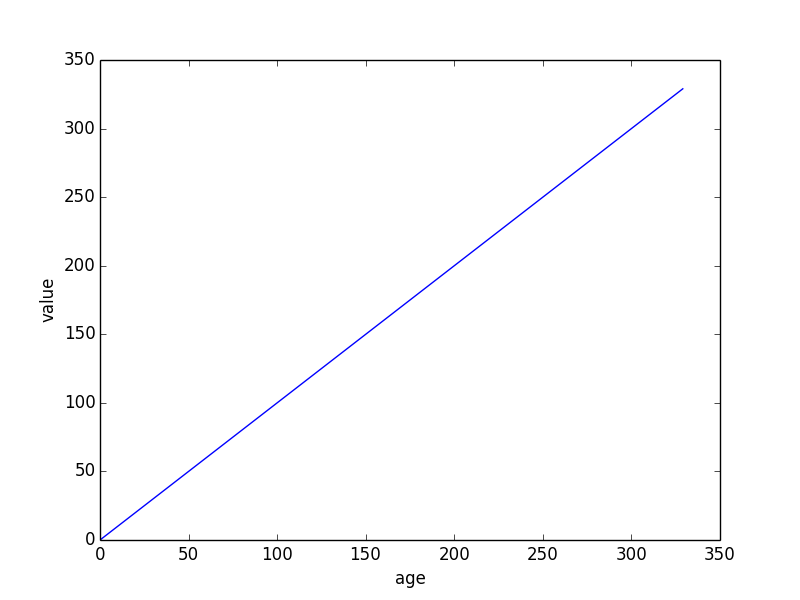
\includegraphics[width=0.5\textwidth]{mru_value}
\caption{policy: mru}
\end{figure}

\begin{equation}
\begin{aligned}
m = 1 - \frac{S}{ed}
\end{aligned}
\end{equation}

\begin{figure}[H]
\centering
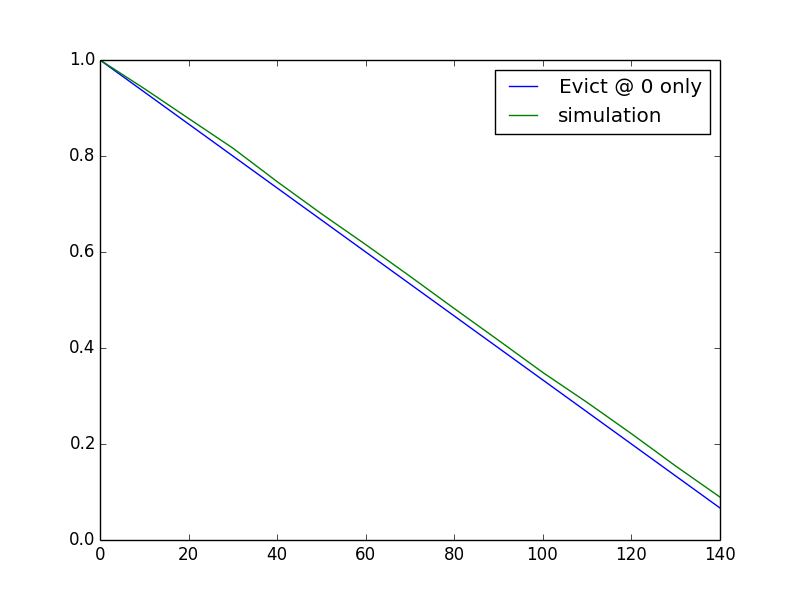
\includegraphics[width=0.5\textwidth]{sim_mru}
\caption{simulation result}
\end{figure}

\subsection{evict at d1}

\begin{figure}[H]
\centering
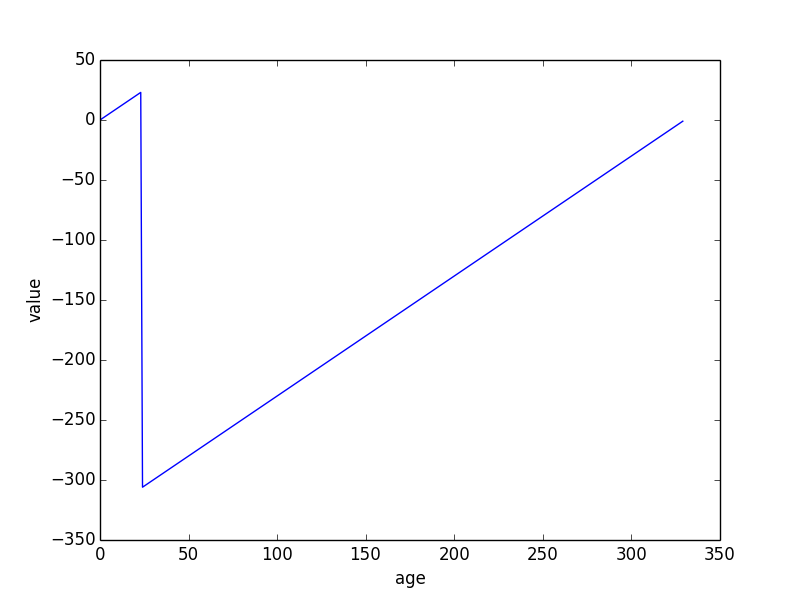
\includegraphics[width=0.5\textwidth]{evict_d1}
\caption{policy: evict candidate at age d1}
\end{figure}

\[
m = \left\{\begin{array}{lr}
      1-p_1 \frac{S}{d_1}, & \text{for } 0 \leq S \leq d_1 \\
      (1-p_1) \frac{ed-S}{ed-d_1}, & \text{for } d_1 \leq S \leq ed
           \end{array}
\]


\subsection{evict at d2, then 0}

\begin{figure}[H]
\centering
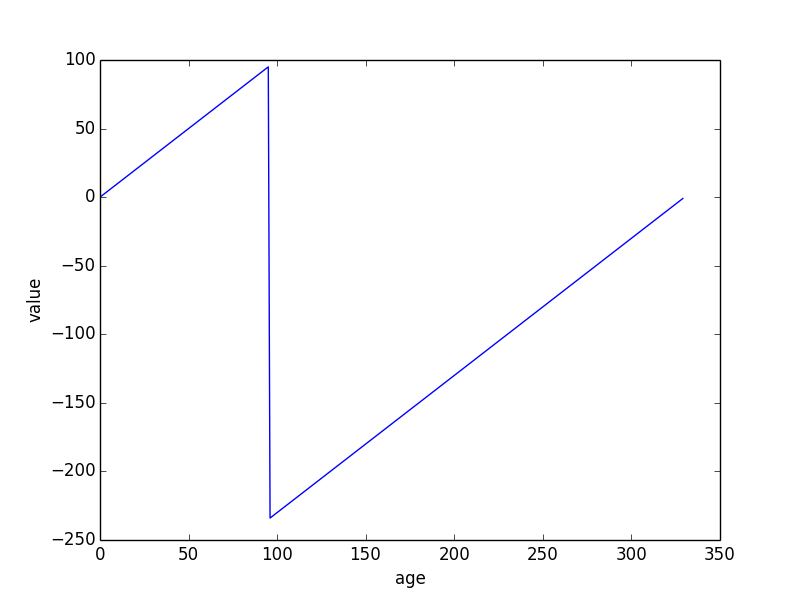
\includegraphics[width=0.5\textwidth]{evict_d2.png}
\caption{replacement policy in value function}
\end{figure}

Let x denote fraction of candidates who make it to the age of d1.

\subsection{Cache behaviors with size between d1 and d2}

\subsubsection{evict at d1}
\label{sec:policyd1}


\begin{center}
\begin{tabular}{c | c c c c}
\hline
events & 1 & d1 & d2 & d3 \\
\hline
hit & & p1 & $p_2 (1-\frac{m}{1-p_1}) $ & $p_3(1-\frac{m}{1-p_1}) $ \\
evict & & m & & \\
\hline
\end{tabular}
\end{center}

\begin{equation}
\begin{aligned}
m = \frac{ed-S}{\frac{p_2}{1-p_1} d_2 + \frac{p_3}{1-p_1} d_3 - d_1}
= (1-p_1) \frac{ed-S}{ed-d_1}
\end{aligned}
\end{equation}

\begin{figure}[H]
\centering
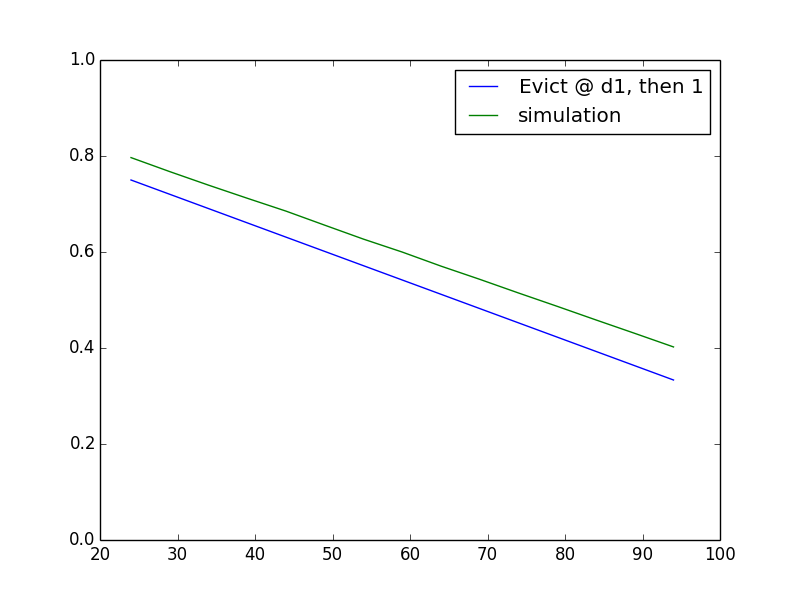
\includegraphics[width=0.5\textwidth]{sim_d1.png}
\caption{simulation result}
\end{figure}

\subsubsection{evict at d2, then 0}

\begin{figure}[H]
\centering
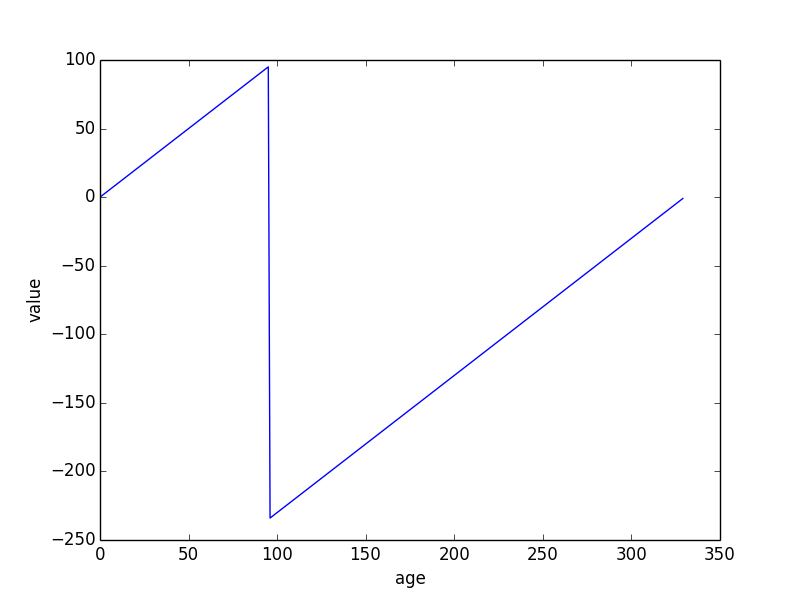
\includegraphics[width=0.5\textwidth]{evict_d2.png}
\caption{replacement policy in value function}
\end{figure}

Let x denote fraction of candidates who make it to the age of d1.

\begin{center}
\begin{tabular}{c | c c c c}
\hline
events & 1 & d1 & d2 & d3 \\
\hline
hit & & $p_1 x$ & $p_2 x$ &  \\
evict & 1-x & & $p_3 x$ & 
\end{tabular}
\end{center}

\begin{equation}
\begin{aligned}
m = 1 - (1-p_3) \frac{S}{p_1 d_1 + p_2 d_2 + p_3 d_2}
\end{aligned}
\end{equation}

\begin{figure}[H]
\centering
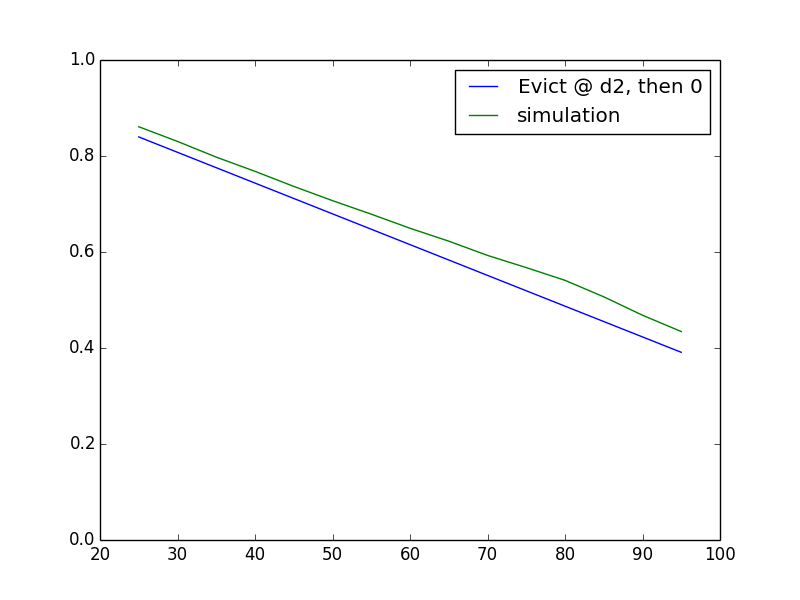
\includegraphics[width=0.5\textwidth]{sim_d2.png}
\caption{simulation result}
\end{figure}

\subsubsection{evict at d2, d1, then 0}

\begin{figure}[H]
\centering
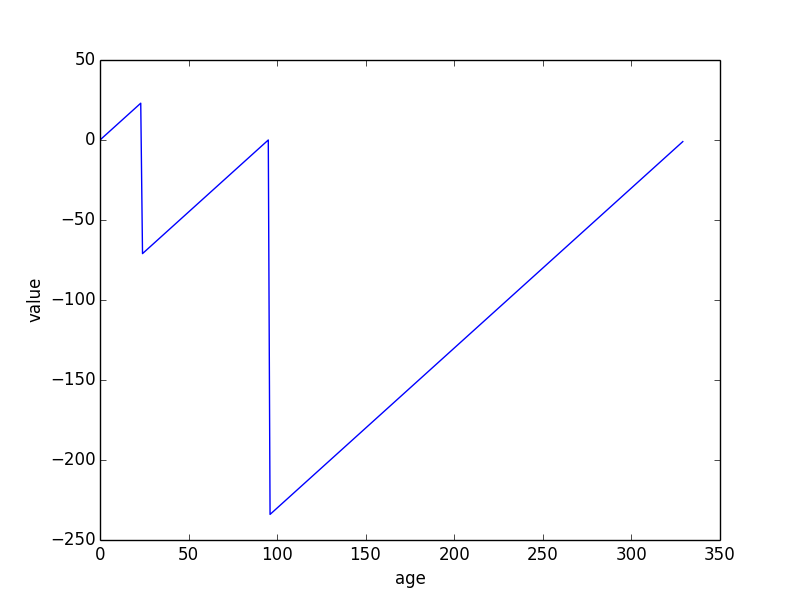
\includegraphics[width=0.5\textwidth]{evict_d2_d1.png}
\caption{replacement policy graph}
\end{figure}

Let x denote fraction of candidates who make it to the age of d1.

\begin{center}
\begin{tabular}{c | c c c c}
\hline
events & 1 & d1 & d2 & d3 \\
\hline
hit & & $p_1 x$ & $p_2 x$ &  \\
evict & & 1-x & $p_3 x$ & 
\end{tabular}
\end{center}

\begin{figure}[H]
\centering
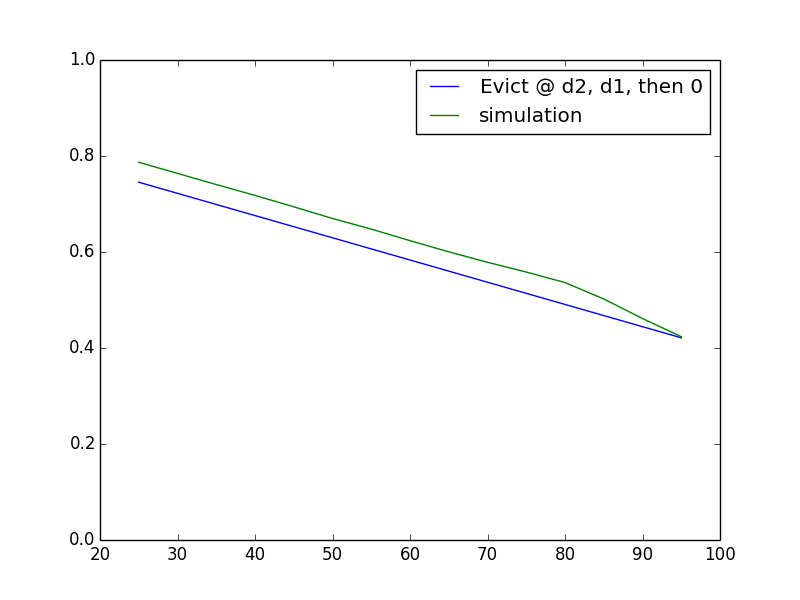
\includegraphics[width=0.5\textwidth]{sim_d2_d1.png}
\caption{simulation result}
\end{figure}

\subsubsection{evict at d1, d2, then 0}

Just behave identical to policy~\ref{sec:policyd1}.

\subsection{Cache behaviors larger then d2}

\subsubsection{evict at d1, then 0}

\begin{center}
\begin{tabular}{c | c c c c}
\hline
events & 0 & d1 & d2 & d3 \\
\hline
hit & & $p_1$& $p_2$ & $p_3-m$ \\
evict & & m &  & 
\end{tabular}
\end{center}

\begin{equation}
\begin{aligned}
m  = (1-p_1) \frac{ed - S}{ed - d_1}
\end{aligned}
\end{equation}

\begin{figure}[H]
\centering
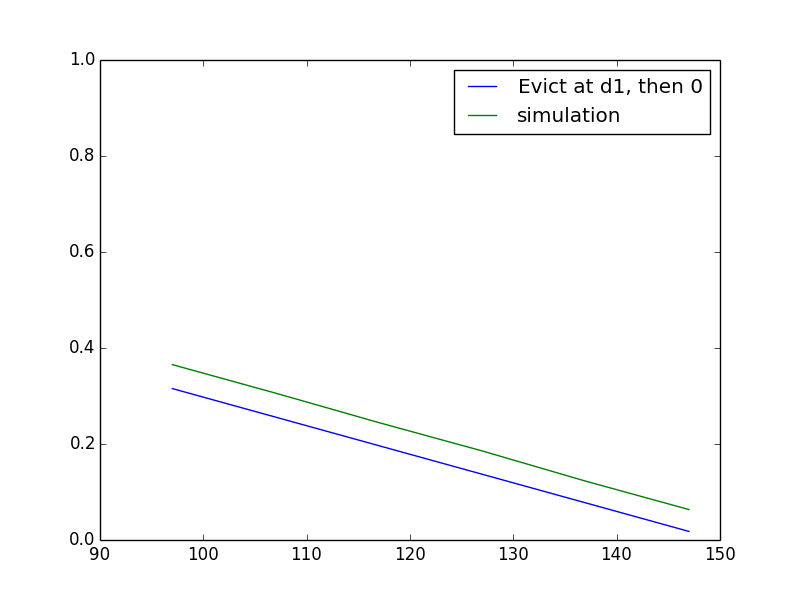
\includegraphics[width=0.5\textwidth]{sim_d1_3.png}
\caption{simulation result}
\end{figure}

\subsubsection{evict at d2, then 0}

\begin{center}
\begin{tabular}{c | c c c c}
\hline
events & 0 & d1 & d2 & d3 \\
\hline
hit & & $p_1$& $p_2$ & $p_3-m$ \\
evict & &  & m & 
\end{tabular}
\end{center}

\begin{equation}
\begin{aligned}
m  = \frac{ed - S}{d_3 - d_2}
\end{aligned}
\end{equation}

\begin{figure}[H]
\centering
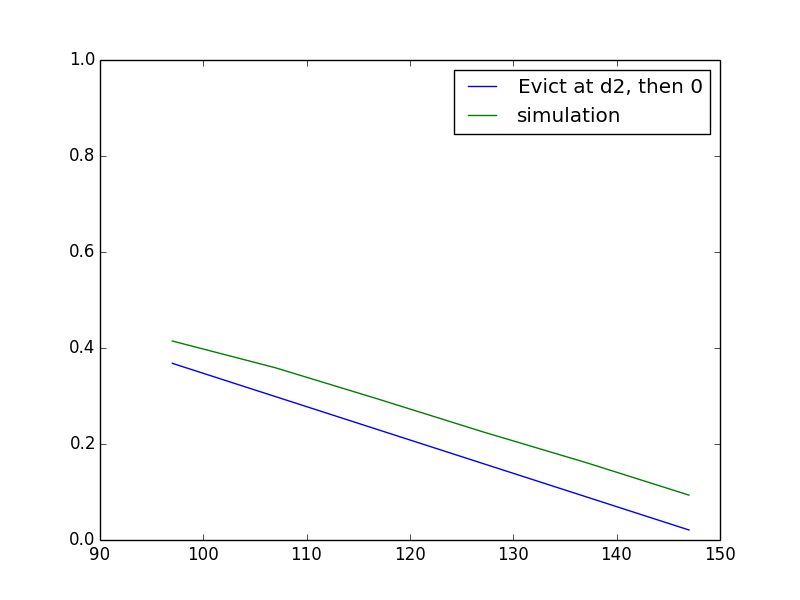
\includegraphics[width=0.5\textwidth]{sim_d2_3.png}
\caption{simulation result}
\end{figure}

\section{Solving MDP with analytical approach}

when $0<a<d_1$:
\begin{equation}
\begin{aligned}
v[a]-v[0] = [(a-1)(1-m)+1][v[1]-v[0]]
\end{aligned}
\end{equation}

when $a=d_1+1$:
\begin{equation}
\begin{aligned}
v[d_1+1]-v[0] = \frac{d_1 (1-m)+1}{1-P_{H}(d_1)}(v[1]-v[0]) - \frac{P_{H}(1-d_1)}{1-P_{H}(d_1)}
\end{aligned}
\end{equation}

% \subsection{Lessons}

\subsubsection{evict at the age of 0}

Note what evicting at age 0 means. It means never replace candidates at all once
the cache is full. So hit rate only depends on the data initially loaded in the
cache due to compulsory miss. 

The probability of being hit at age $d_1$ becomes expected number of array items
within the cache $\times$ expected time the item is referenced again: $p_1 S
\times \frac{1}{d_1}$. The same calculation applies to hit at $d_2$.

The overall events:

\begin{center}
\begin{tabular}{ c | c c c c }
\hline
 	&	0 & d1  & d2 & d3\\ 
\hline
 hit &	  & $\frac{p_1 S}{d_1}$ & $\frac{p_2 S}{d_2}$  &\\  
 evict &	m &    & &\\
\hline
\end{tabular}
\end{center}

Then we have this miss rate function of cache size:

\begin{equation}
1-m = \frac{p_1 S}{d_1} + \frac{p_2 S}{d_2} + \frac{p_3 S}{d_3}
\end{equation}

Note that this equation is different from what we have in bimodal analysis. I
think this is the right one. Confirmed by simulation and cache trace analysis.

\subsubsection{Evict at d1, then 0}
\label{sec:d1-0}

Note: This policy, with other policies that favors $d_2$ or $d_1$ totally makes
no sense in my simulation. It took me a few days to realize the problem, which
is I generate access pattern based on counter, i.e. for the trimodal simulation
I just iterate three arrays in order. This rigorously exact order means every
time the policy evicts an candidate, say it from array 2, the piece of new data
put into cache is also from array 2. You can think of it as doing LRU for array
2.  The same reason apply for array3. So these policies just make no sense
without randomness. This is how I screwed it up.

This also means in order to make policies that favor $d_1$ or $d_2$ really make
sense in simulation, randomness has to be introduced to access pattern. By doing
this, the simulated cache trace won't help me come up with an analytical model,
but could determine the best policy under different scenarios.

Given the mistakes I have made when trying to come up with an analytical model
for the trimodal RDD, I think a more effective approach to examine if the value
iteration could yield the optimal policy is to directly run the random
simulation. By random I mean when generating the access pattern, simulator uses
weighted choice instead of iteration in exact order. 

Next is to use value iteration to compute optimal policy and see if it's
consistent with the simulation result. The important part, I guess, is to have
the initial parameters: RDD, cache size, hit rate, hit age distribution,
eviction age distribution, consistent with each other. By consistent I mean that
the hit rate, hit age distribution and eviction age distribution should be
consistent with RDD, cache size, and initial policy (not necessarily be
optimal). 

One straight way to guarantee the consistency of these initial parameters is to
run a simulation and collect the data, but that makes the init parameters a bit
complicated. Fortunately the policy of evicting at 0 is relatively easy to come
up with an analytical model, seen by the following section.

So I could use `evict at 0' policy model to compute the miss rate, hit age
distribution, and eviction age distribution as input.

\subsection{Simulation}

Setup:
\begin{center}
\begin{tabular}{ c | c c c}
\hline
array id & x(size) & p(reference probability) & d(reuse distance) \\
\hline
1 & 4 & 0.4 & 10 \\
2 & 8 & 0.4 & 20 \\
3 & 16 & 0.2 & 80 \\
\hline
\end{tabular}
\end{center}

\begin{figure}[H]
\centering
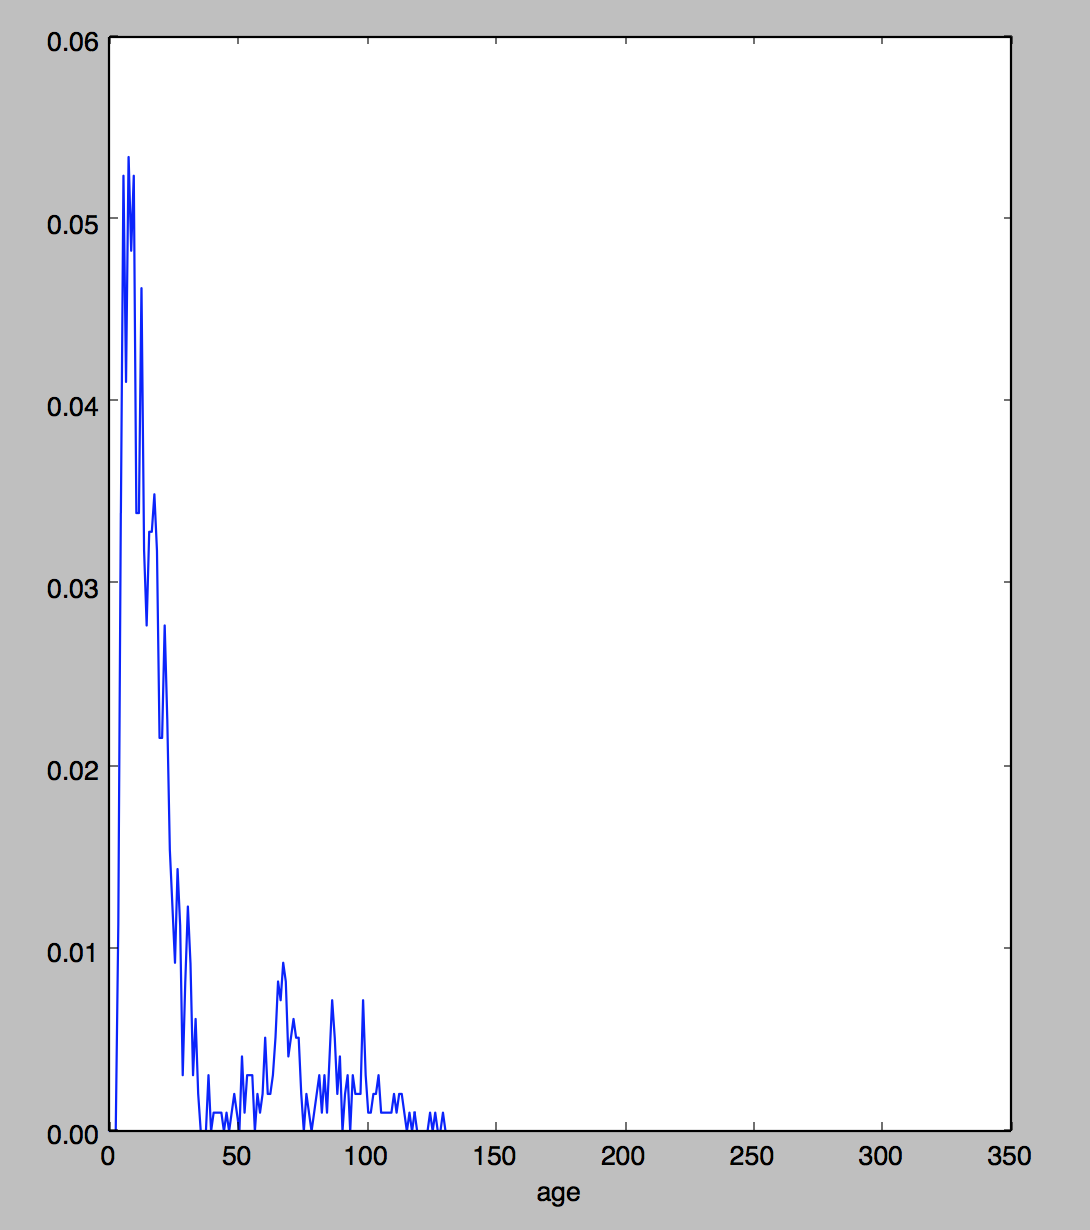
\includegraphics[width=0.5\textwidth]{trimodal-rdd-random-1.png}
\caption{rdd of simulation}
\end{figure}

Simulation tells that the optimal policy is to evict at $d_2$, then 0.

Then I use the data calculated based on the modal in section~\ref{sec:d1-0} as
the input of value iteration. 

What Value iteration gives:
\begin{figure}[H]
\centering
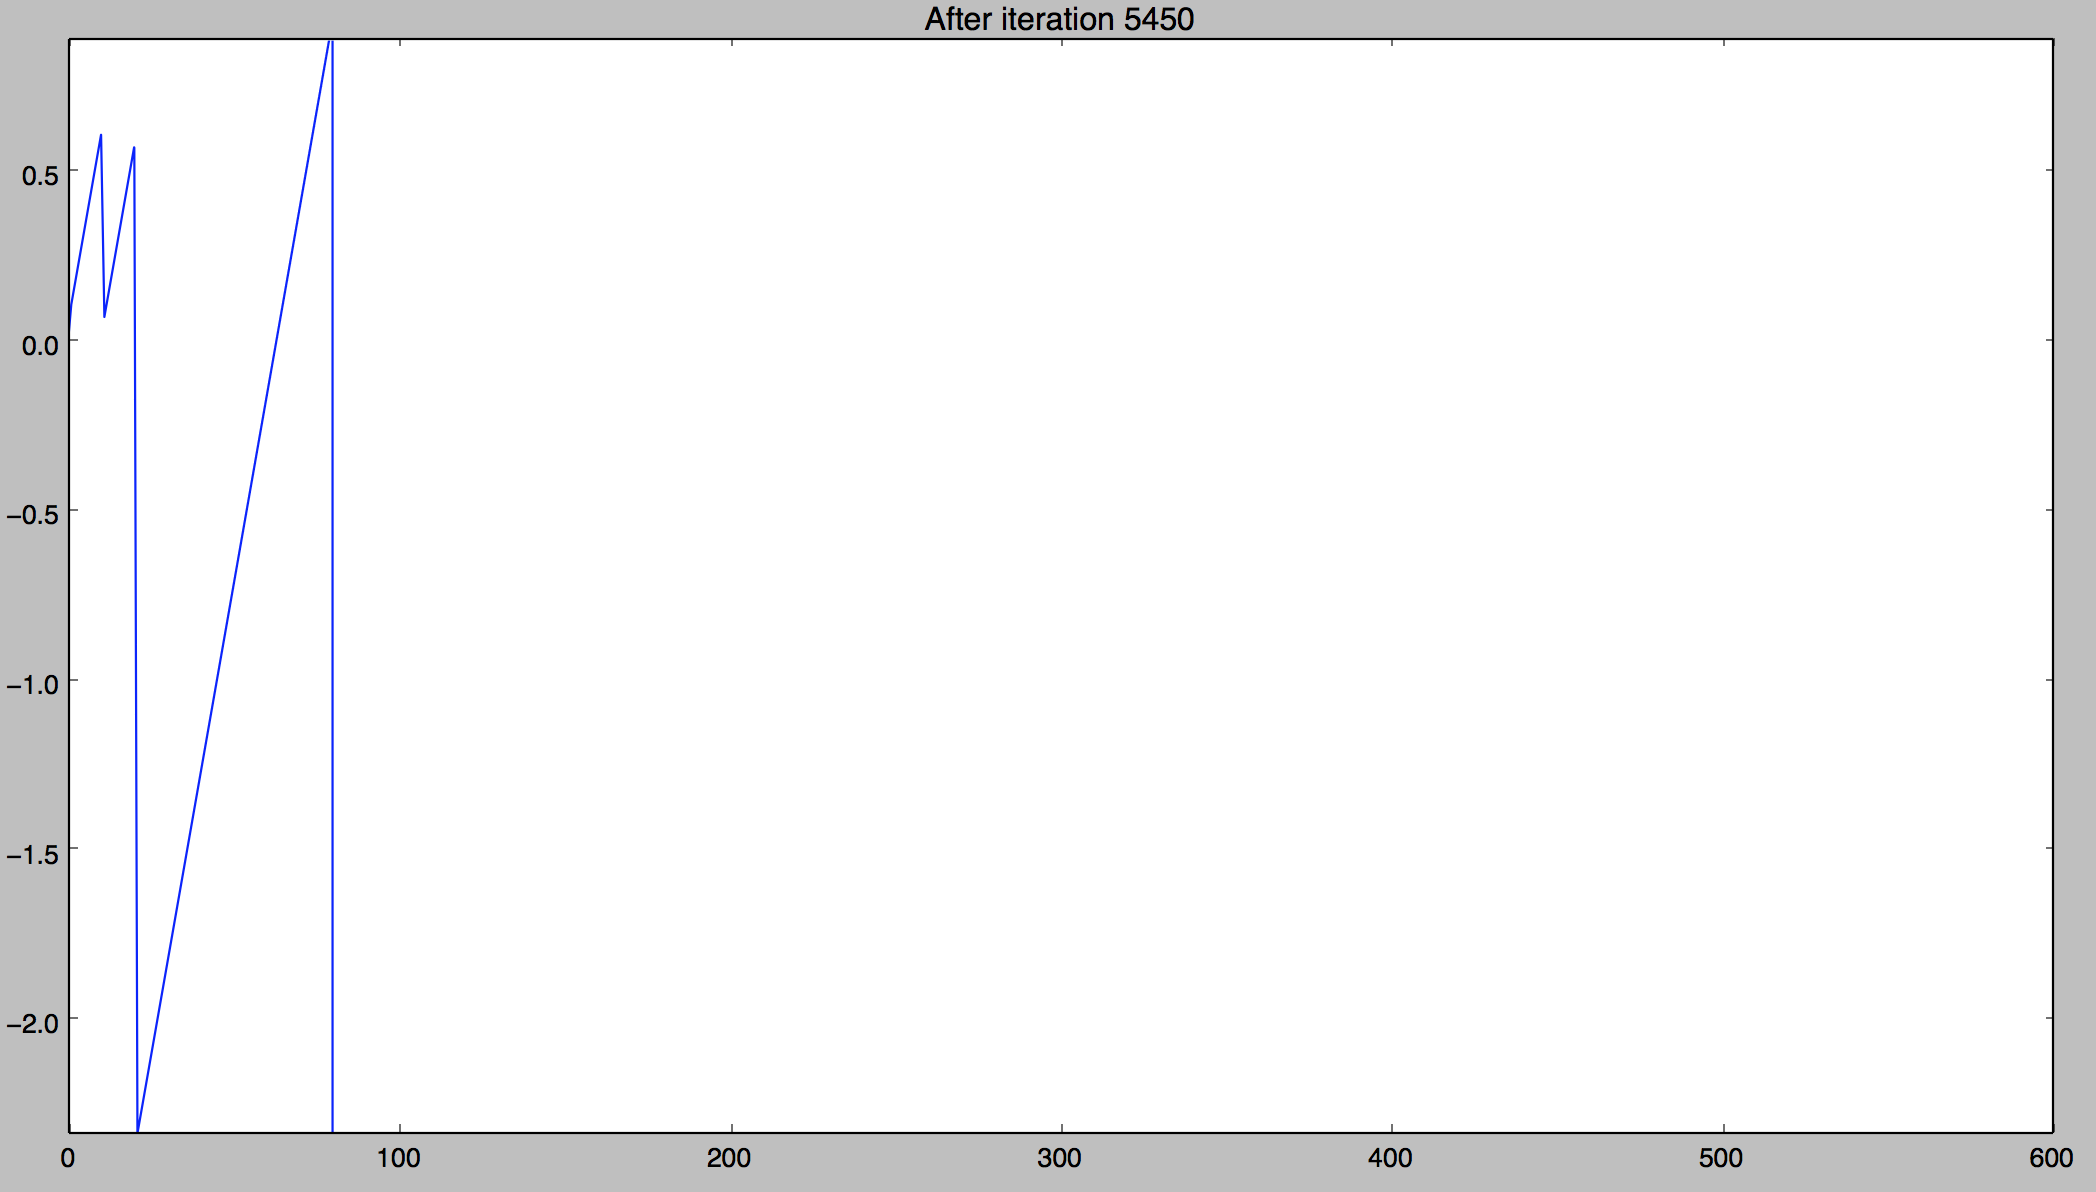
\includegraphics[width=0.8\textwidth]{vi-output-1.png}
\caption{value iteration output}
\end{figure}

Seems consistent with simulation result.

However, when I changed the simulation parameter into:

\begin{center}
\begin{tabular}{ c | c c c}
\hline
array id & x(size) & p(reference probability) & d(reuse distance) \\
\hline
1 & 8 & 0.4 & 20 \\
2 & 28 & 0.4 & 70 \\
3 & 32 & 0.2 & 160 \\
\hline
\end{tabular}

\begin{figure}[H]
\centering
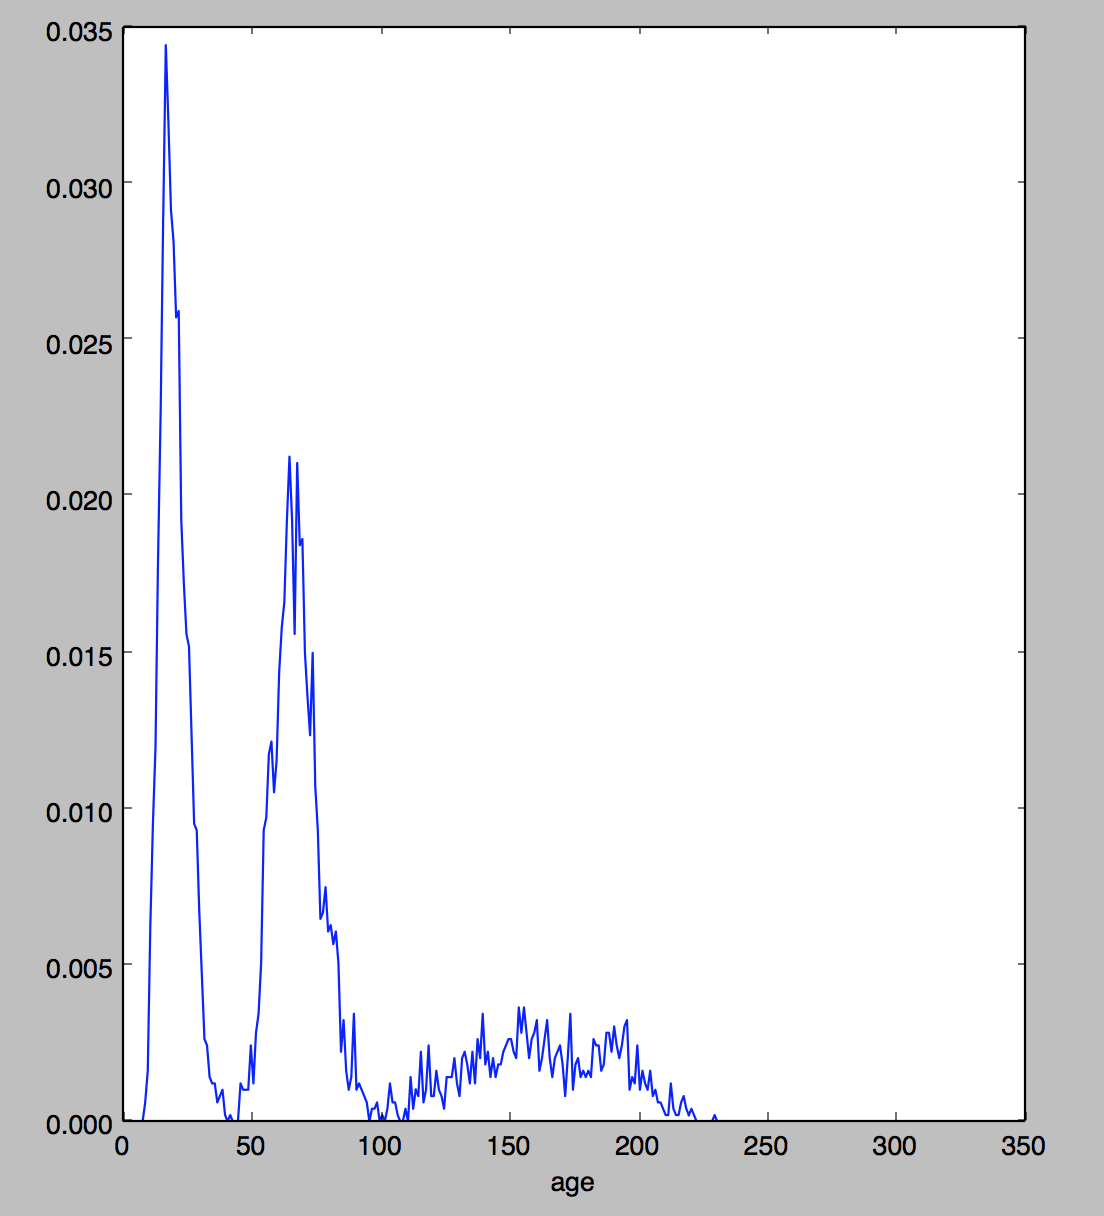
\includegraphics[width=0.5\textwidth]{trimodal-rdd-random-2.png}
\caption{rdd of simulation}
\end{figure}
\end{center}

Simulation result shows the optimal policy is still evict d2, then 0.

But what Value iteration gives become :
\begin{figure}[H]
\centering
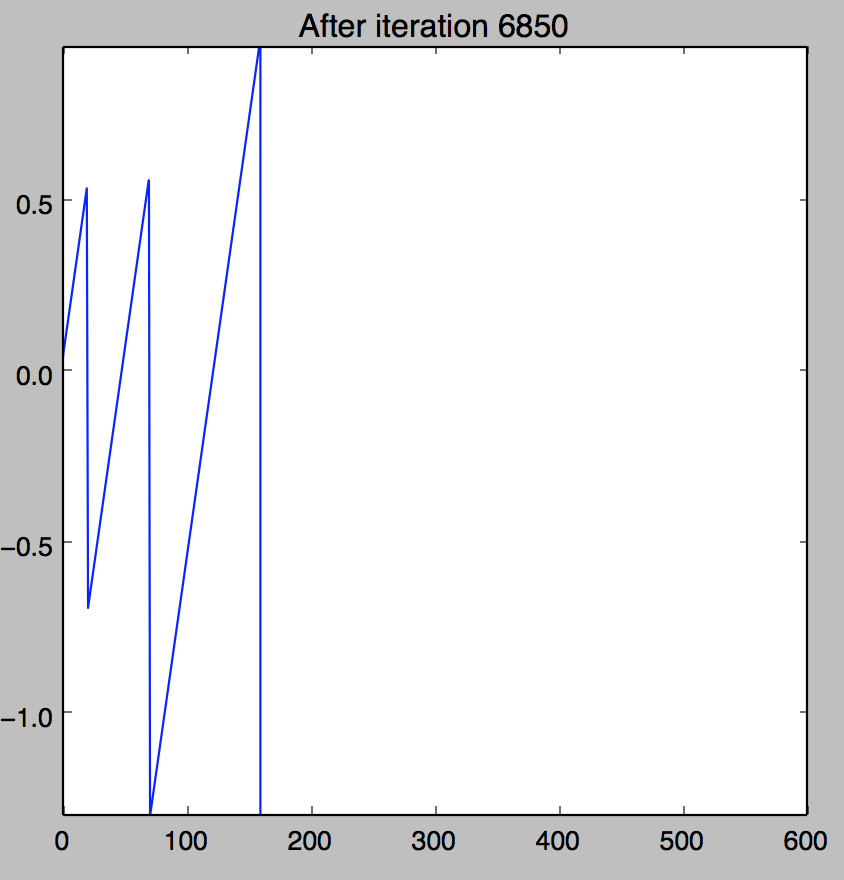
\includegraphics[width=0.8\textwidth]{vi-output-2.png}
\caption{value iteration output}
\end{figure}

Not consistent with simulation result.


\end{document}
